\documentclass[10pt]{article}

\usepackage[english]{babel}
\usepackage[utf8x]{inputenc}
\usepackage[fleqn]{amsmath}
\usepackage{amssymb}
\usepackage{amsfonts}
\usepackage{graphicx}
\usepackage[ruled,linesnumbered,noend]{algorithm2e}
\usepackage{empheq}
\usepackage{float}
\usepackage{enumitem}
\usepackage{tikz}
\usepackage[colorlinks=true,urlcolor=blue]{hyperref}

\DeclareMathOperator*{\argmin}{arg\, min}

\title{Introduction to Machine Learning, Fall 2014 - Exercise session V}
\author{Rodion ``rodde'' Efremov \\ 013593012}

\begin{document}
 \maketitle

\color{blue}
\section*{Problem 1 (3 points)}
Consider the following two sets of 80 cars each: Set `A' consists of 10 Volvos, 25 Toyotas, and 45 Audis, while set `B' consists of 8 Volvos, 32 Toyotas, and 40 Audis. Which set do you intuitively think is more pure (that is, has lower impurity), and why? Compute the entropy, the Gini index, and the misclassification error for each of the two sets. According to these measures, which set is more pure? Could this phenomenon (conflict among the measures) happen if there were just two classes (two types of car) rather than three? Why, or why not?

\color{black}
To me, it seems that the set `A' is more pure than `B', for ``intervals'' in set `A' are more ``equal'' than in the set `B'.

The entropy of the set A is ($\log = \log_2$)
\begin{align*}
&-\frac{10}{80} \log \frac{10}{80} - \frac{25}{80} \log \frac{25}{80} - \frac{45}{80} \log \frac{45}{80} \\ 
&= \frac{1}{8}(\log 80 - \log 10) +\frac{5}{16} (\log 80 - \log 25) + \frac{9}{16} (\log 80 - \log 45) \\
 &\approx 0.375 + 0.524 + 0.467 \\
 &\approx 1.366.
\end{align*}

The entropy of the set B is
\begin{align*}
&-\frac{8}{80} \log \frac{8}{80} - \frac{32}{80} \log \frac{32}{80} - \frac{40}{80} \log \frac{40}{80} \\
&= \frac{1}{10} \log 10 + \frac{4}{10} (\log 80 - \log 32) + \frac{1}{2} \log 2 \\
&\approx 0.332+ 0.529 + 0.5 \\
&\approx 1.361.
\end{align*}

The Gini index of the set A is
\begin{align*}
&1 - \Bigg( \frac{10}{80} \Bigg)^2 - \Bigg( \frac{25}{80} \Bigg)^2 - \Bigg( \frac{45}{80}  \Bigg)^2 \\
&= 1 - (1 / 8)^2 - (5/16)^2 - (9/16)^2 \\
&\approx 1 - 0.016 - 0.098 - 0.316 \\
&\approx 0.570.
\end{align*}

The Gini index of the set B is
\begin{align*}
&1 - \Bigg( \frac{8}{80} \Bigg)^2 - \Bigg( \frac{32}{80} \Bigg)^2 - \Bigg( \frac{40}{80} \Bigg)^2 \\
&\approx 1 - 0.01 - 0.16 - 0.25 \\
&\approx 0.58.
\end{align*}

The classification error of the set A is
\begin{align*}
1 - \frac{45}{80} = 1 - \frac{9}{16} = 0.4375.
\end{align*}

The classification error of the set B is
\begin{align*}
1 - \frac{40}{80} = 0.5.
\end{align*}

In summary:
\begin{table}[h]
\centering
\begin{tabular}[H]{|c||c|c|c|}
\hline
 & Entropy & Gini index & Classification error \\
 \hline
 A & 1.366 & 0.570 & 0.438 \\
 \hline
 B & 1.361 & 0.580 & 0.5 \\
 \hline
\end{tabular}
\end{table}
According to the above table, the set A is slightly more pure than B.

Suppose a set contains $N$ elements in total, and $M$ of them belong to one type of elements and $N - M$ to the other one. Now, all the impurity measure will attain their maximum value at around $M = \frac{N}{2}$, and all measures will be monotonically increasing on $[0, \frac{N}{2})$, and monotonically decreasing on $(\frac{N}{2}, N]$, so improvement in, say, Gini index will lead to improvement in classification error or entropy, and vice versa. (As can be seen in a figure of course slides.)

\color{blue}
\section*{Problem 2 (3 points)}
Consider a binary classification problem with the following set of attributes and attribute values:
\begin{itemize}
  \item Air conditioner = \{ Working, Broken \}
  \item Engine = \{ Good, Bad \}
  \item Mileage = \{ High, Medium, Low \}
  \item Rust = \{ Yes, No \}
\end{itemize}
Suppose a rule-based classifier produces the following rule set:
\begin{itemize}
  \item (Mileage = High) $\leftarrow$ (Value = Low)
  \item (Mileage = Low) $\leftarrow$ (Value = High)
  \item ((Air conditioner = Working) and (Engine = Good)) $\leftarrow$ (Value = High)
  \item ((Air conditioner = Working) and (Engine = Bad)) $\leftarrow$ (Value = Low)
  \item (Air conditioiner = Broken) $\leftarrow$ (Value = Low)
\end{itemize}
Given the above, answer the following:
\begin{enumerate}
  \item[(a)] Are the rules mutually exclusive?
  \color{black} Yes, they are. On each record, at most one rule is triggered.
  
  \color{blue}
  \item[(b)] Is the rule set exhaustive? 
  \color{black} Suppose that Mileage = Medium. This is not covered by two first rules, but it all boils down to the fact that Air conditioner will ``catch'' all the records regardless of the state of Engine. So, yes, the rule set is exhaustive.

  \color{blue}
  \item[(c)] Is ordering needed for this set of rules?
  \color{black} No, it doesn't appear that way: mileage is a good predictor of the value of a car, so it is justified to have the first two rules where they are.
  
  \color{blue}
  \item[(d)] Do you need a default class for the rule set?
  \color{black}
  No, we don't need that since the rules are exhaustive.
\end{enumerate}

\color{blue}
\section*{Problem 3 (3 points)}
Given a set of $N$ points $y_1, \dots, y_N$, with each $y_i \in \mathbb{R}$, show that...
\begin{itemize}
  \item[(a)] ... the value $y^{\ast}$ which minimizes the sum of \textit{squared} errors, i.e.
 \[
 y^{\ast} = \underset{\hat{y}}{\argmin} \sum_{i = 1}^N (y_i - \hat{y})^2
 \]
 is given by the \textit{mean} of the $y_i$, i.e. $y^\ast = \sum_i y_i / N$.
 
 \color{black} 
 Suppose we have 
 \[
 \sum_{i = 1}^N (y_i - t)^2 = \sum_{i = 1}^N (y_i^2 - 2y_it + t^2).
 \]
 Now the first derivative of the above sum with respect to $t$ is given by
 \[
 \sum_{i = 1}^N 2t - 2y_i,
 \]
 and the second derivative of the same sum is given by
 \[
 \sum_{i = 1}^N 2 = 2N > 0.
 \]
 The original sum is, therefore, minimized (2nd derivative $> 0$) at point, where the first derivative is zero, i.e.
 \begin{align*}
 \sum_{i = 1}^N 2t - 2y_i &= 0 \\
 \sum_{i = 1}^N t - y_i &= 0 \\
 Nt &= \sum_{i = 1}^N y_i \\
 t &= \frac{\sum_{i = 1}^N y_i}{N},
 \end{align*}
 which proves that the mean of the $y_i$ minimizes the sum of squared errors.
 
 \color{blue}
 \item[(b)] ... the value $y^{\ast}$ which minimizes the sum of \textit{absolute} errors, i.e.
 \[
 y^\ast = \underset{\hat{y}}{\argmin} \sum_{i = 1}^N |y_i - \hat{y}|
 \] 
 is given by the \textit{median} of the $y_i$. [Hint for part (b): Break the sum into parts corresponding to \textit{pairs} of observations, pairing the smallest with the largest point, the second-smallest with the second-largest point, etc.]
 
 \color{black}
 Suppose the $y_i$ are sorted so that $y_1 \leq y_2 \leq \dots \leq y_N$. Let us rephrase the sum. If $N$ is even, we have
 \begin{align*}
 \sum_{i = 1}^N |y_i - \hat{y}| &= \sum_{i = 1}^{N / 2} |y_i - \hat{y}| + |y_{N + 1 - i} - \hat{y}|
 \end{align*}
 Basically this means that as to keep the sum of absolute errors at its minimum, $\hat{y} \in [y_1, y_N]$, because whenever that is the case, $|y_1 - \hat{y}| + |y_N - \hat{y}|$ is minimized and equals $y_N - y_1$. If we go ``outside'' that range, the sum above becomes $y_N - y_1 + 2\min(|\hat{y} - y_N|, |\hat{y} - y_1|) > |y_1 - \hat{y}| + |y_N - \hat{y}|$. Also, we must restrict $\hat{y}$ to $[y_2, y_{N - 1}], [y_3, y_{N -2}]$ and so on. If $N$ is odd, the sum of absolute errors is minimized whenever $\hat{y} \in [y_{\lfloor N / 2 \rfloor + 1}, y_{\lfloor N / 2 \rfloor + 1}]$, which implies $\hat{y} = y_{\lfloor N / 2 \rfloor + 1}$; by assumption of $y_i$'s being sorted, $y_{\lfloor N / 2 \rfloor + 1}$ is the median. In the case of even $N$, the strongest constraint on value of $\hat{y}$ is the interval $I = [y_{N / 2}, y_{N / 2 + 1}]$, where the two values are medians. In fact, any $\hat{y} \in I$ minimizes the sum of absolute errors as it does not ``leave'' from any interval $[y_1, y_N], [y_2, y_{N - 1}], \dots$.
\end{itemize}

\color{blue}
\section*{Problem 4 (15 points)}
In this problem, we will test linear regression on a simple synthetic dataset. We will use the following polynomial as the underlying target function
\[
y = f(x) = 2 + x - 0.5 x^2.
\]
First, randomly sample 30 points $x_i$ from the uniform distribution on the interval $[-3,3]$. Then, randomly generate the $y_i$ using
\[
y_i = f(x_i) + n_i,
\]
where $f$ is as defined above, and the $n_i$ are i.i.d. normal random variables with zero mean and standard deviation 0.4. The resulting 30 pairs $(x_i, y_i)$ is your data set for this exercise.
\begin{itemize}
  \item[(a)] First, let's fit polynomials of order 0 to 10 to this dataset using linear regression, minimizing the sum of squares error. That is, fit functions of the form
  \[
  \hat{y} = \sum_{p = 0}^K w_px^p
  \]
  with $K = 0, \dots, 10$ to the data. For instance, for $K = 4$ the polynomial to fit is 
  \[
  \hat{y} = w_0 + w_1x + w_2x^2 + w_3x^3 + w_4x^4.
  \]
  For each of the 11 values of $K$, produce a separate plot showing the datapoints $(x_i, y_i)$ and the fitted polynomial. (Plot the polynomial as a curve, in the full interval $[-3, 3]$, overlayed on the scatterplot of the points.) You should see that as the order of the polynomial $K$ increases, the curve comes closer and closer to fitting all the datapoints. For each value of $K$, calculate the coefficient of determination $R^2$ and comment on the behaviour of this measure as a function of $K$.
  
  \color{black}
  First of all, run a declaration of $R^2$ stuff:
  \begin{verbatim}
  run('rsquared.m');
  \end{verbatim}
  which is defined as
  \begin{verbatim}
  function [r] = rsquared(xs, ys)
    ssres = 0;
    sstot = 0;

    mean_x = mean(xs);

    for i = 1:length(xs)
        sstot += (xs(i) - mean_x)^2;
        ssres += (xs(i) - ys(i))^2;
    end

    r = 1 - ssres / sstot;
  end
  \end{verbatim}
  As to generate the 30 $x_i$, let us type
  \begin{verbatim}
  xs = unifrnd(-3, 3, 1, 30);
  \end{verbatim}
  Next, let us declare the function $f$:
  \begin{verbatim}
  f = @(x) 2 + x - 0.5 * x^2
  \end{verbatim}
  Create the $y_i$ vector:
  \begin{verbatim}
  ys = zeros(1, 30);
  for i = 1:30
    ys(i) = f(xs(i)) + normrnd(0, 0.4);
  end
  \end{verbatim}
  Now, data is here. Next
  \begin{verbatim}
  for K = 0:10
    figure;
    plot(xs, ys, 'o');
    hold on;
    p = polyfit(xs, ys, K);
    xt = linspace(-3, 3);
    fs = polyval(p, xt);
    fs2 = polyval(p, xs);
    plot(xt, fs, 'r-');
    title(["K = ", num2str(K), " R-squared = ", num2str(rsquared(xs, fs2))]);
    legend('Data points', 'Fitting polynomial', 'location', 'southwest');
  end
  \end{verbatim}    
  
  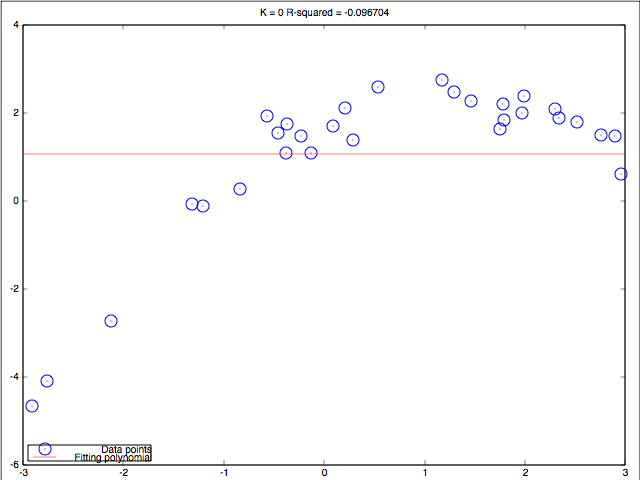
\includegraphics[width=\textwidth,height=\textheight,keepaspectratio]{K0}
  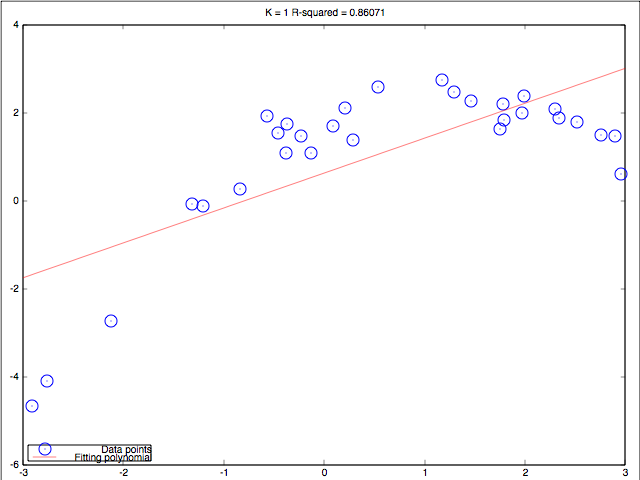
\includegraphics[width=\textwidth,height=\textheight,keepaspectratio]{K1}
  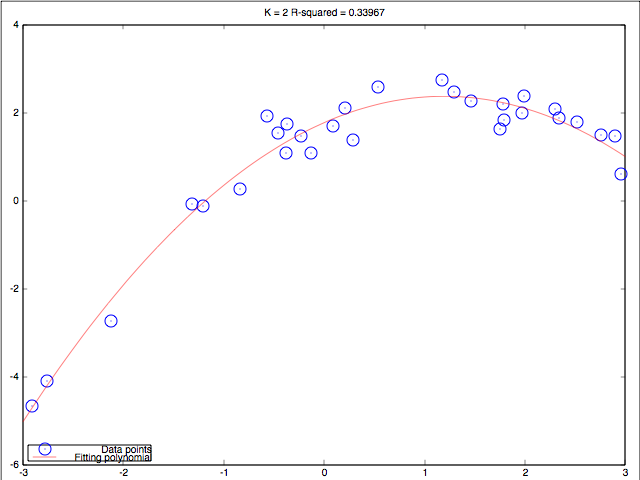
\includegraphics[width=\textwidth,height=\textheight,keepaspectratio]{K2}
  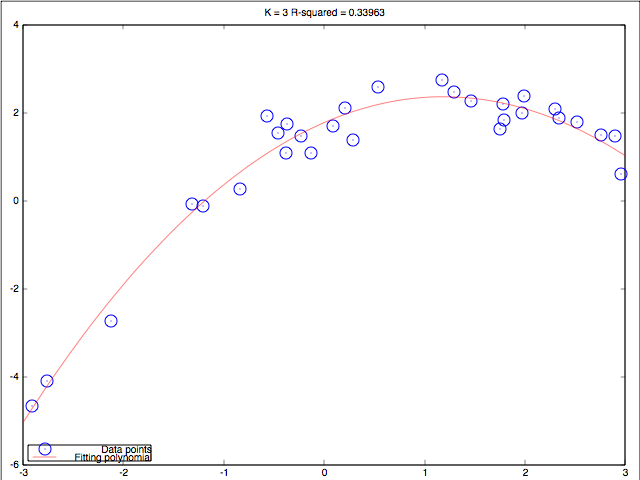
\includegraphics[width=\textwidth,height=\textheight,keepaspectratio]{K3}
  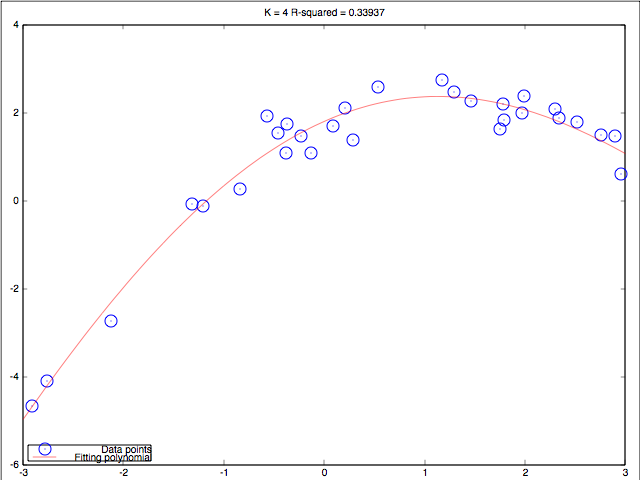
\includegraphics[width=\textwidth,height=\textheight,keepaspectratio]{K4}
  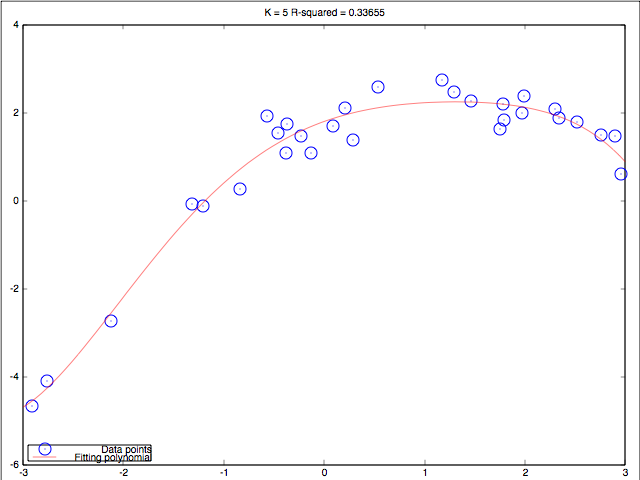
\includegraphics[width=\textwidth,height=\textheight,keepaspectratio]{K5}
  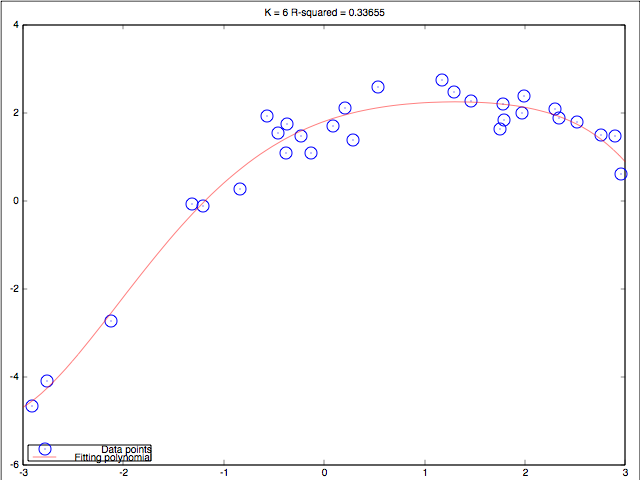
\includegraphics[width=\textwidth,height=\textheight,keepaspectratio]{K6}
  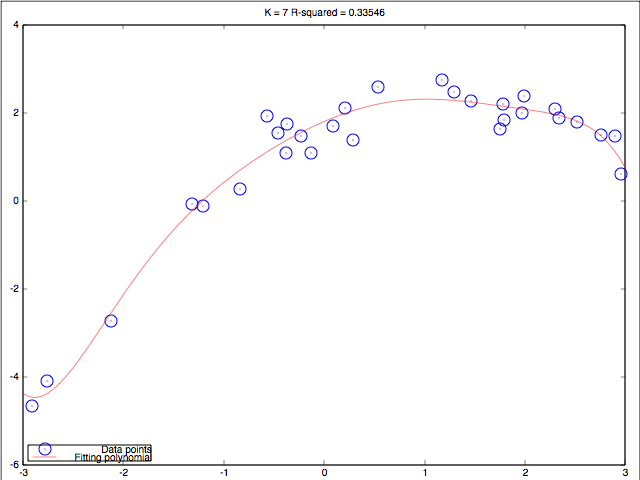
\includegraphics[width=\textwidth,height=\textheight,keepaspectratio]{K7}
  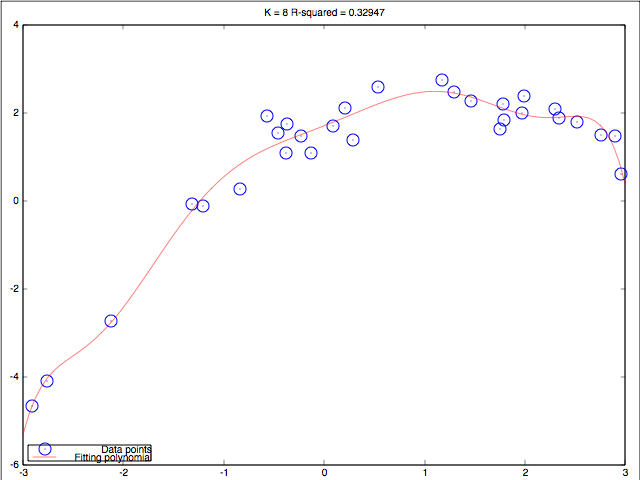
\includegraphics[width=\textwidth,height=\textheight,keepaspectratio]{K8}
  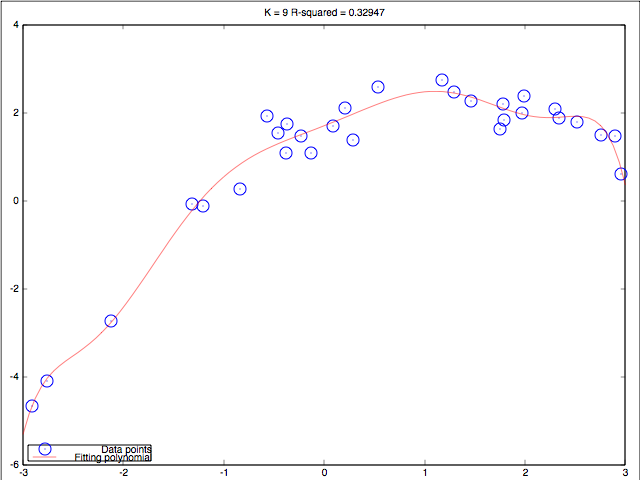
\includegraphics[width=\textwidth,height=\textheight,keepaspectratio]{K9}
  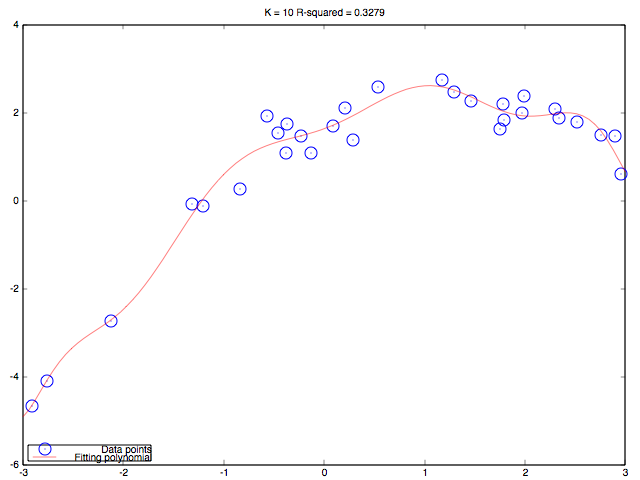
\includegraphics[width=\textwidth,height=\textheight,keepaspectratio]{K10}
  
  As can be seen from the images above, the $R^2$ attains its maximum value at $K = 1$, after which it is strictly decreasing, and it seems like its rate of ``growth'' is similar to $C - \log K$, for some $C$.
  \color{blue}
  \item[(b)] Finally, let's test model selection based on 10-fold cross-validation. That is, divide the dataset into 10 equal-sized subsets (i.e. 3 datapoints in each subset), and, for each value of $K = 0, \dots, 11$ and each data subset $j = 1, \dots, 10$, use all the data except the data in subset $j$ to fit the polynomial of order $K$, and compute the resulting sum of squared errors on subset $j$. For each value of $K$, sum together the errors coming from the different $j$. Plot these results with $K$ on the horizontal axis, and the sum of squared errors on the vertical axis. How does this function behave? Does the cross-validated error improve with increasing $K$? Which $K$ gives the minimum error, and what are the corresponding estimated coefficients? Compare them to the true coefficients used in $f(x)$ to generate the data.
  
  \color{black}
  Now, let us split the data:
  \begin{verbatim}
  xsplit = zeros(10, 3);
  ysplit = zeros(10, 3);
  for i = 1:10
    xsplit(i,:) = xs( 3 * (i - 1) + 1 : (i - 1) * 3 + 3);
    ysplit(i,:) = ys( 3 * (i - 1) + 1 : (i - 1) * 3 + 3);
  end
  \end{verbatim}
  The rest is given by:
  \begin{verbatim}# For the error sums.
errs = zeros(1, 12);

# Stored polynomial coefficients.
coefs = zeros(12, 12);

# For each value of K, do...
for K = 0:11
    printf("--- K = %d.\n", K);
    # For each subset, do...
    for j = 1:10
        # Copy the data points.
        xdata = xs;
        ydata = ys;
        # Obtain the jth subset.
        xjth = xdata(3 * (j - 1) + 1 : 3 * (j - 1) + 3);
        yjth = ydata(3 * (j - 1) + 1 : 3 * (j - 1) + 3);
        # Remove the jth subset.
        xdata(3 * (j - 1) + 1 : 3 * (j - 1) + 3) = [];
        ydata(3 * (j - 1) + 1 : 3 * (j - 1) + 3) = [];
        # Fit a polynomial of degree K over the datapoints.
        p = polyfit(xdata, ydata, K);
        # Add the coefficients.
        for kk = 0:K
            coefs(K + 1, kk + 1) += p(kk + 1) / 12;
        end
        # Evaluate the jth subset.
        fjth = polyval(p, xjth);
        err = sum_of_squared_errors(fjth, yjth);
        printf('Sum of squared errors on %dth subset is %f.\n', j, err);
        errs(K + 1) += err;
    end
    # Print the error sum.
    printf("-- Error sum is %f. ", errs(K + 1));
    # Print the coefficients of the polynomial.
    printf("Coefficients: ");
    for kk = 0:K
        printf("%f ", coefs(K + 1,kk + 1));
    end
    printf("\n");
end

# Prepare to plot K-to-error graph.
Ks = zeros(1, 12);
for K = 0:11
    Ks(K + 1) = K;
end
figure
plot(Ks, errs);
end
  \end{verbatim}
  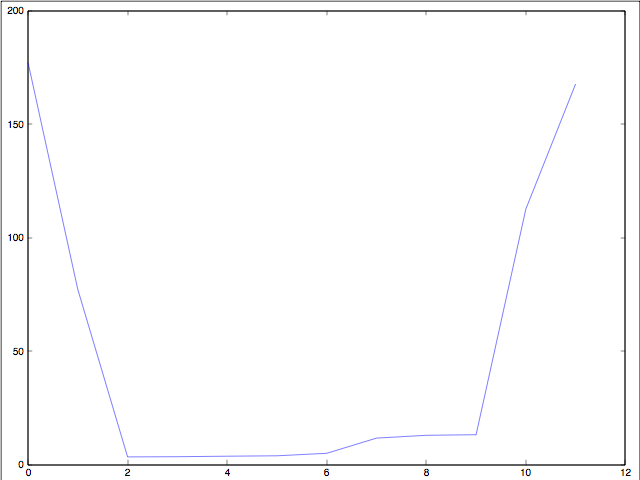
\includegraphics[width=\textwidth,height=\textheight,keepaspectratio]{KsVersusErrors}
  It can be seen that the error function decreases rapidly from $K = 0$ to $K = 2$, where it approximately attains the minimum value, which carried over to $K = 4$, after which it start to grow towards higher values of $K$ until it reaches $K = 9$, where things go out of control. (Depends on random number generator: sometimes values on the right side of plot do not ``blow out.'')
  
  Increasing the $K$ does not pay off after $K = 4$. The sums of squared errors is minimized at $K = 2$, where the average coefficients over all $j$s are $1.76, 0.841, -0.452$, which resemble the coefficients $2, 1, -0.5$.
  
\end{itemize}

\end{document}